\section{Method}

\subsection{Task definition}
Given a Vietnamese comment $x$, the model predicts six binary pragmatic labels: implicit sentiment, sarcasm, irony, idiom/figurative language, code-switching, and mocking. It also predicts a three-way polarity label and a seven-way emotion label. Binary macro-F1 is the mean of the negative- and positive-class F1 values; macro-pragmatic F1 is the mean of the six binary macro-F1 values.

The operational definitions were informed by a Vietnamese dictionary and published linguistic accounts of verbal irony and code-switching \citep{vien-ngon-ngu-hoc-hoang-phe-1994,burgers-etal-2011,ghosh-etal-2018-sarcasm,poplack-1980}. Implicit sentiment is evaluative stance without an overt sentiment expression; for annotation, irony denotes a broader incongruity between literal and intended evaluation, whereas sarcasm is a target-directed, derisive or taunting realization of such incongruity; idiom/figurative language denotes a conventional idiom or another nonliteral/figurative expression; code-switching alternates Vietnamese with material from another language; and mocking directs derision at a target. These are operational labels and may co-occur.

\subsection{XLM-R-large multi-task model}

\begin{figure*}[t]
  \centering
  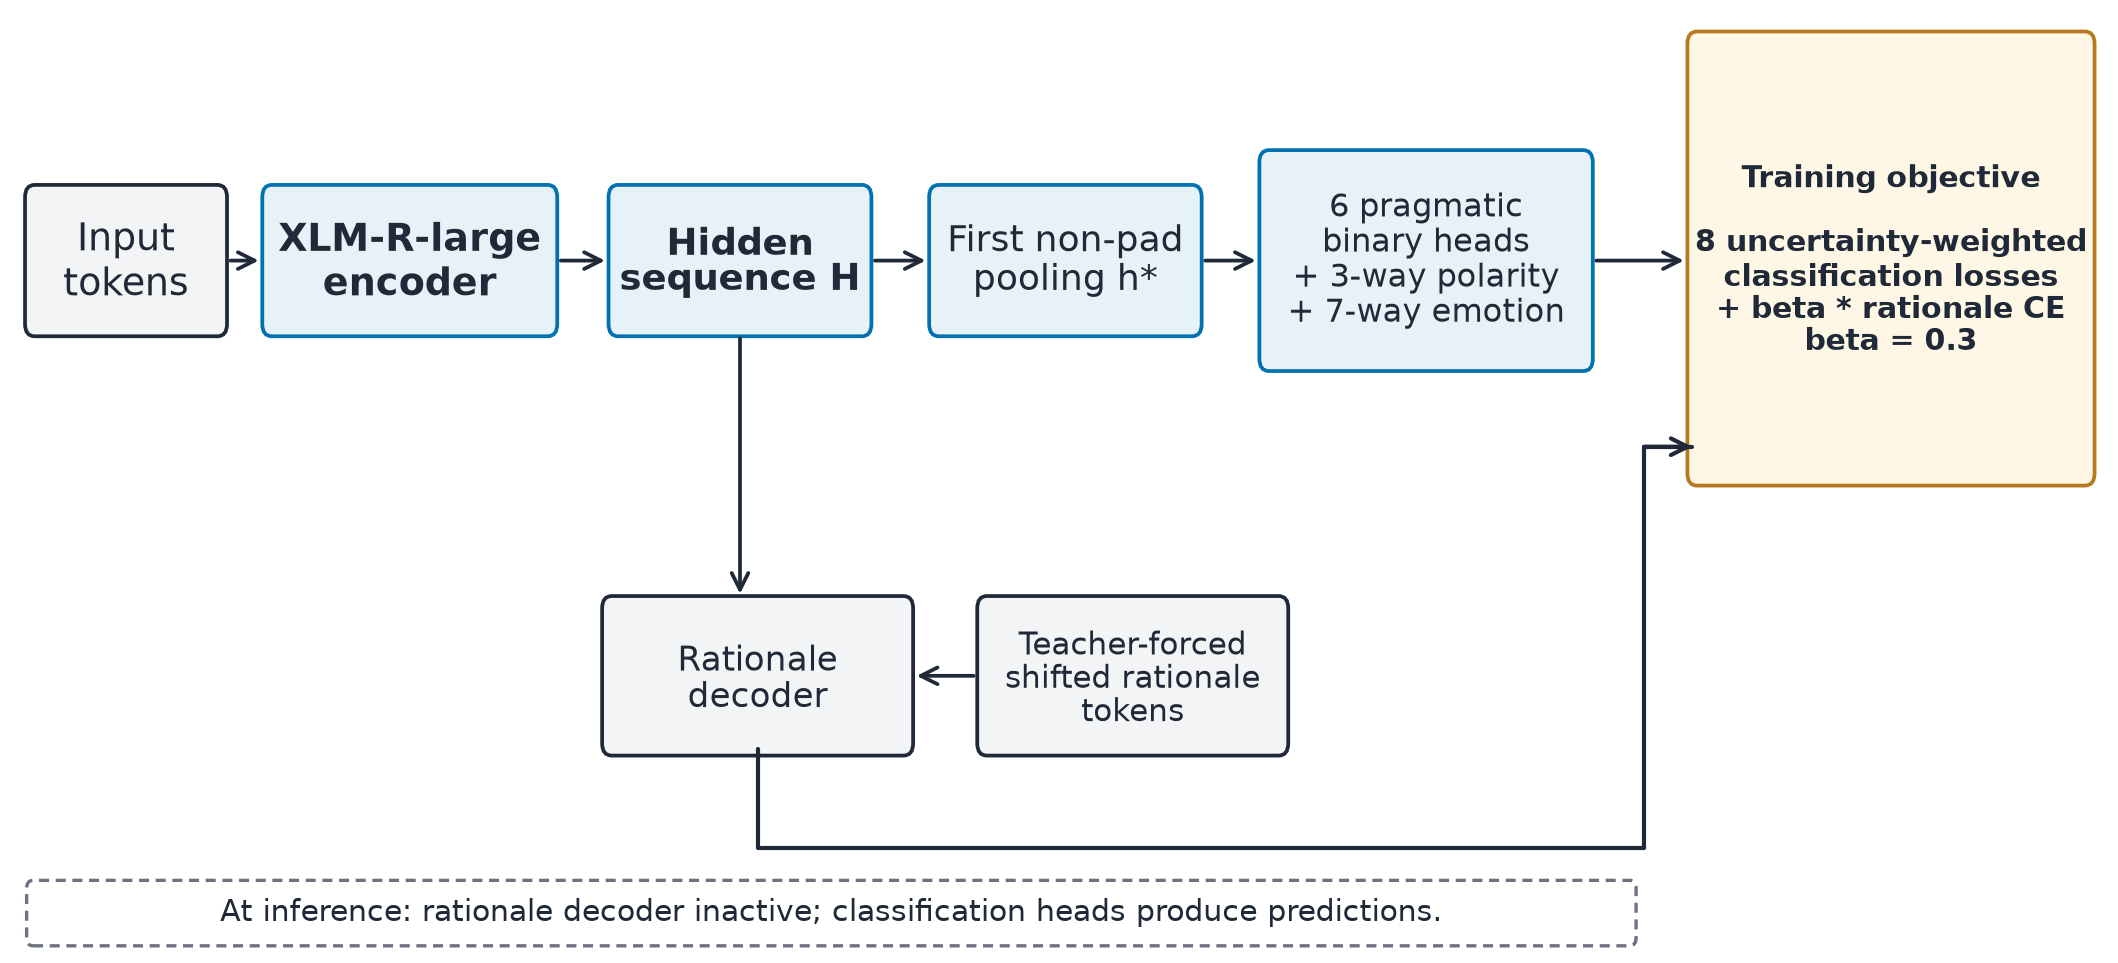
\includegraphics[width=\textwidth]{figures/figure_architecture_schematic.png}
  \caption{Proposed XLM-R-large multi-task architecture.}
  \label{fig:architecture}
\end{figure*}

Our proposed XLM-R-large multi-task model uses \texttt{Facebook\allowbreak{}AI/xlm-r\allowbreak{}oberta-l\allowbreak{}arge}. It pools the first nonpadding hidden state, applies dropout 0.1, and feeds task-specific linear heads: six one-logit pragmatic heads, one three-logit polarity head, and one seven-logit emotion head. These classification heads are the inference interface.

The six pragmatic heads use weighted binary cross-entropy with logits; polarity and emotion use class-weighted cross-entropy. Let $\mathcal{T}$ be the eight classification tasks, $m_t$ a task multiplier, $\ell_t$ an unweighted task loss, and $s_t$ its learned log variance. Multipliers are applied before uncertainty weighting:

\[
\begin{aligned}
s_t^{\mathrm{c}}=\operatorname{clip}(s_t,-5,5), \\
\mathcal{L}_{\mathrm{cls+rat}}=\sum_{t\in\mathcal{T}}\Bigl[\tfrac12 e^{-s_t^{\mathrm{c}}}(m_t\ell_t)+\tfrac12s_t^{\mathrm{c}}\Bigr] \\
{}+\beta\mathcal{L}_{\mathrm{rat}},\qquad \beta=0.3.
\end{aligned}
\]
For the primary model, the fixed task multipliers are 1.01 for implicit sentiment, 1.01 for sarcasm, 1.05 for irony, 1.04 for code-switching, and 1.00 for idiom/figurative language, mocking, polarity, and emotion. All class weights are computed from the training split only: each pragmatic positive weight is $N_k^-/N_k^+$, while each class in the three-way polarity and seven-way emotion heads receives $N/(C N_c)$, where $N$ is the training count, $C$ is the number of classes, and $N_c$ is the count for class $c$.

The rationale module is a two-layer autoregressive \texttt{TransformerDecoder} with causal masking, hidden size 128, four attention heads, feed-forward size 512, and dropout 0.1. Teacher forcing gives the rationale token loss. Rationale targets are truncated at 160 tokens.

\subsection{Training and rationale supervision}
Training uses maximum sequence length 128, AdamW ($2\times10^{-5}$ learning rate; weight decay 0.01), at most 10 epochs, bf16, physical batch size 8 with four accumulation steps (effective batch size 32), gradient clipping 1.0, cosine scheduling, warmup ratio 0.20, and early-stopping patience 10. The seeds are 20260521, 20260522, and 20260523. The selected checkpoint maximizes development macro-pragmatic F1. Each pragmatic threshold is selected on development data from 0.05 to 0.95 in increments of 0.01, with ties resolved toward 0.5. The final task multipliers were inherited from controlled pilot variants rather than from an exhaustive grid search, and beta=0.3 was fixed in the final training protocol. For the reported final runs, checkpoint and threshold selection used development data only, and test evaluation was performed after the development-stage configuration was frozen.

For training examples, 7,998 rationale targets were generated by the GPT-4.1-mini deployment (model version 2025-04-14) \citep{openai-2025-gpt41-mini}. The fixed instruction was ``Generate a rationale for this Vietnamese comment:'', followed by the Vietnamese comment; gold labels were excluded. Generation used temperature 0 and a maximum of 256 output tokens. Rationale supervision is training-only: the rationale decoder is discarded at inference and produces no deployed output.
